\section{SuperCaps}
\begin{minipage}[lt]{10cm}
	{\footnotesize \begin{tabular}[c]{ | p{3cm} | p{6cm} |}
	    	\hline
	    	voltage		  & $\sim 2~V$ \\
	    	\hline
	    	capacity	  & $\sim 3000~F$ \\
	    	\hline
	    	power density & $P' = \frac{U_{SCAPmax} \cdot I}{m} \frac{U_{SCAPmax}^2}{4 \cdot R_s \dot m} \quad m =$ Masse\\
	    	\hline
	    	energy		  & $W' = \frac{1}{2 \cdot m} \cdot C \cdot U_{SCAPmax}^2$ \\
	    	 & $\rightarrow U = \sqrt{\frac{2 \cdot E}{C}}$\\
	    	\hline
	    	efficiency	  & $\eta = \frac{R_L}{R_L + R_S} \rightarrow$ max @$50\%: R_L = R_S$ \\
	    	 & $\eta = \frac{U - R_S \cdot I}{U} = \frac{P - R I^2}{P}$ \\
	    	\hline
	\end{tabular}}
\end{minipage}
\begin{minipage}[rt]{7cm}
	\centering
	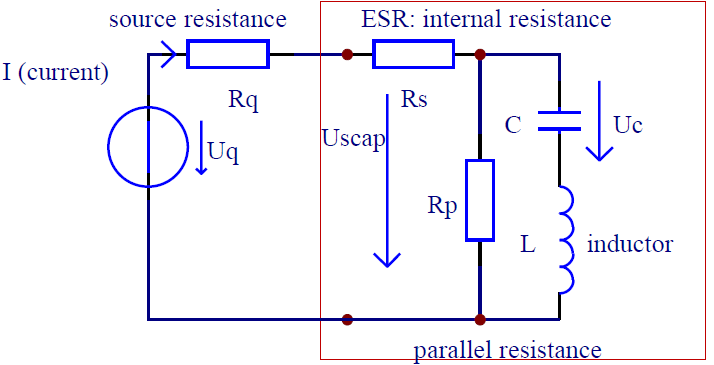
\includegraphics[width=0.9\textwidth]{./images/SCAP_real.png}
	\captionof{figure}{Real model for a SCAP}
\end{minipage}
\begin{figure}[h!]
	\centering
  	\begin{subfigure}[t]{0.49\textwidth}
		\centering
		\adjustbox{width=\textwidth}{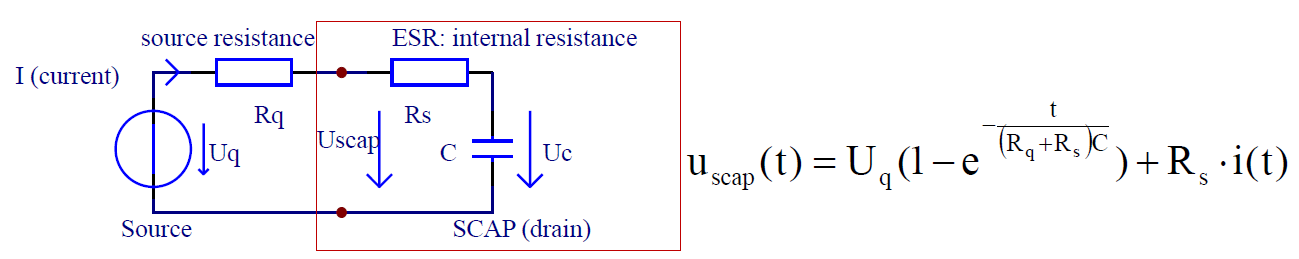
\includegraphics{./images/SCAP_laden.png}}
	   	\caption{charging}
	\end{subfigure}
	\begin{subfigure}[t]{0.49\textwidth}
	 	\centering
	    \adjustbox{width=\textwidth}{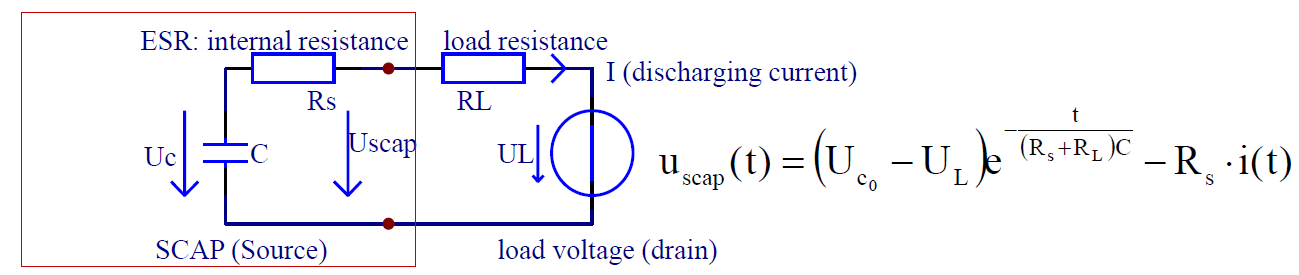
\includegraphics{./images/SCAP_entladen.png}}
	    \caption{discharging}
	\end{subfigure}
	\caption{Simplified model for a SCAP}
\end{figure}

